% mn2eguide.tex
% v2.1 released 03/05/2002
%
% Adapted from mnguide.tex
% v1.3 released 14th September 1995
% v1.2 released 5th September 1994 (M. Reed)
% v1.1 released 18th July 1994
% v1.0 released 28th January 1994

% The journal style files and macros, with guides on their use, are
% available by anonymous FTP on the Internet from the Comprehensive
% TeX Archive Network (CTAN) sites ftp.tex.ac.uk and ftp.dante.de.
% The files are in the directories
% /tex-archive/macros/plain/contrib/mnras and
% /tex-archive/macros/latex209/contrib/mnras for the TeX and LaTeX
% files respectively.


\documentclass[useAMS,usenatbib]{mn2e}

\title[Monthly Notices: \LaTeXe\ guide for authors]
  {Monthly Notices of the Royal Astronomical
  Society: \\ \LaTeXe\ style guide for authors}
\author[A. Woollatt et al.]
  {A.~Woollatt,$^1$\thanks{Affiliated to ICRA.}
  M.~Reed,$^1$ R.~Mulvey,$^1$ K.~Matthews,$^1$
  D.~Starling,$^1$ Y.~Yu,$^1$
  \newauthor % starts a new line in the
             % author environment
  A.~Richardson,$^1$
  P.~Smith,$^2$\thanks{Production Editor.}
  N. Thompson$^2$\footnotemark[2]
  and G. Hutton$^2$\footnotemark[2] \\
  $^1$Cambridge University Press, Shaftesbury
      Road, Cambridge CB2 2BS\\
  $^2$Blackwell Publishing,
      23 Ainslie Place, Edinburgh EH3 6AJ}
\date{Released 2002 Xxxxx XX}

\pagerange{\pageref{firstpage}--\pageref{lastpage}} \pubyear{2002}

\def\LaTeX{L\kern-.36em\raise.3ex\hbox{a}\kern-.15em
    T\kern-.1667em\lower.7ex\hbox{E}\kern-.125emX}

\newtheorem{theorem}{Theorem}[section]

\begin{document}

\label{firstpage}

\maketitle

\begin{abstract}
 This guide is for authors who are preparing papers for
 \textit{Monthly Notices of the Royal Astronomical Society} using the
\LaTeXe\ document preparation system and the {\tt mn2e} class file.
\end{abstract}

\begin{keywords}
 \LaTeXe\ -- class files: \verb"mn2e.cls"\ -- sample text -- user guide.
\end{keywords}

\section{Introduction}

The standard format for papers submitted to \textit{Monthly
Notices} is \LaTeXe. The layout design for \textit{Monthly
Notices} has been implemented as a \LaTeXe\ class file. The {\tt
mn2e} class file is based on the {\tt mn} style file, which in
turn is based on \verb"article" style as discussed in the \LaTeX\
manual \citep{la}. Commands that differ from the standard \LaTeX\
interface, or that are provided in addition to the standard
interface, are explained in this guide. This guide is not a
substitute for the \LaTeX\ manual itself. We also refer authors to
\citet{kd} and \citet{kn}. Authors planning to submit their papers
in \LaTeX\ are advised to use \verb"mn2e.cls" as early as possible
in the creation of their files.

\subsection{The mn2e document class}

The use of \LaTeX\ document classes allows a simple change of class to
transform the appearance of your document. The {\tt mn2e} class file
preserves the standard \LaTeX\ interface such that any document that can be
produced using the standard \LaTeX\ \verb"article" class can also be
produced with the {\tt mn2e} class file. However, the measure (or width of
text) is narrower than the default for \verb"article", and even narrower
than for the \verb"A4" style, therefore line breaks will change and long
equations may need re-setting.

When your article is printed in the journal, it is typeset in 9/11~pt
Times Roman. As most authors do not have this font, it is likely that the make-up
will change with the change of font. For this reason, we ask you to ignore
details such as slightly long lines, page stretching, or figures falling
out of synchronization, because these details can be dealt with at a later
stage.

\subsection{General style issues}

For general style issues, authors are referred to the `Instructions for
 Authors' on the journal web page.\footnote{http://www.blackwell-science.com/mnr/}
Authors who are interested in the details of style are referred to
\citet{bu} and \citet{ch}. The language of the journal is British
English and spelling should conform to this.

Use should be made of symbolic references (\verb"\ref") in order to
protect against late changes of order, etc.

\subsection{Submission of \LaTeXe\ articles to the journal}

Authors should refer to the journal web page for instructions on how to
submit a new manuscript for refereeing, and on how to supply the files for
an accepted paper to Blackwell Publishing. Abbreviated instructions are
also available on the inside back cover of the journal. Note that the
standard procedure is to supply a PDF file at submission stage and
\TeX/\LaTeX\ file(s) of the text plus EPS files of the figures at
acceptance stage. If for some reason you cannot do this, please notify the
RAS as soon as possible.

The correct \textit{Monthly Notices} House Style should be used --
again, details are given in the Instructions for Authors on the
journal web page\footnotemark[1] and in the Style Guide published
in the 1993 January 1 issue (\mbox{MNRAS}, 260, 1). Ensure that
any author-defined macros are gathered together in the file, just
before the \verb"\begin{document}" command.

\section{Using the mn2e class file}

If the file \verb"mn2e.cls" is not already in the appropriate system
directory for \LaTeX\ files, either arrange for it to be put there or copy
it to your working directory. The {\tt mn2e} document class is implemented
as a complete class, {\em not\/} a document style option. In order to use
the MN document class, replace \verb"article" by \verb"mn2e" in the
\verb"\documentclass" command at the beginning of your document:
%
\begin{verbatim}
\documentclass{article}
\end{verbatim}
%
is replaced by
%
\begin{verbatim}
\documentclass{mn2e}
\end{verbatim}
%
In general, the following standard document style options should {\em
not\/} be used with the {\tt mn2e} class file:
%
\begin{enumerate}
  \item {\tt 10pt}, {\tt 11pt}, {\tt 12pt} -- unavailable;
  \item {\tt twoside} (no associated style file) -- {\tt
     twoside} is the default;
  \item {\tt fleqn}, {\tt leqno}, {\tt titlepage} --
        should not be used (\verb"fleqn" is already incorporated into
        the MN style);
  \item {\tt twocolumn} -- is not necessary as it is the default style.
\end{enumerate}
%

The {\tt mn2e} class file has been designed to operate with the standard
version of \verb"lfonts.tex" that is distributed as part of \LaTeX. If you
have access to the source file for this guide, \verb"mn2eguide.tex", and to
the specimen article, \verb"mn2esample.tex", attempt to typeset both of
these. If you find font problems you might investigate whether a
non-standard version of \verb"lfonts.tex" has been installed in your
system.

Authors using \LaTeX\ wishing to create PDF files with smooth
fonts are advised to read Adobe FaxYI Document Number 131303 by
Kendall Whitehouse. Type 1 PostScript versions of the Computer
Modern fonts are now freely available and are normally installed
with new \TeX/\LaTeX\ software. Information is available from
Y\&Y.\footnote{http://www.yandy.com/resources.htm} Alternatively,
you may wish to use Times font when creating your PDF file, e.g.\\
\begin{verbatim}
\documentclass[useAMS]{mn2e}
\usepackage{times}
\end{verbatim}

\subsection{Additional document style options}

The following additional style options are available with the {\tt mn2e}
class file:
\begin{description}
  \item {\tt onecolumn} -- to be used {\it only} when two-column output
        is unable to accommodate long equations;
  \item {\tt landscape} -- for producing wide figures and tables which
        need to be included in landscape format (i.e.\ sideways) rather
        than portrait (i.e.\ upright). This option is described below.
  \item {\tt doublespacing} -- this will double-space your
        article by setting \verb"\baselinestretch" to 2.
  \item {\tt referee} -- 12/20pt text size, single column,
        measure 16.45~cm, left margin 2.75~cm on A4 page.
  \item {\tt galley} -- no running heads, no attempt to align
        the bottom of columns.
  \item \verb"useAMS" -- this enables the production of upright Greek
characters $\upi$, $\umu$ and $\upartial$.

    \item \verb"usedcolumn" -- this uses the package file \verb"dcolumn.sty"
to define two new types of column alignment for use in tables.

    \item \verb"usenatbib" -- this uses Patrick Daly's \verb"natbib.sty"
package for cross-referencing.

 \item \verb"usegraphicx" -- this enables the use of the {\tt graphicx}
 package for inclusion of figures. Note that the standard \LaTeX\
 graphics package \verb"graphicx.sty" is
 required in order to use the \verb"usegraphicx" option.
\end{description}

Please place any additional command definitions at the very start
of the \LaTeX\ file, before the \verb"\begin{document}".
Author-defined macros should be kept to a minimum. Please do not
customize the MNRAS macros or class file, or redefine macros that
are already in the class file, and please do not include
additional definitions unless they are actually used in the paper.

\subsection{Landscape pages}

If a table or illustration is too wide to fit the standard measure, it must
be turned, with its caption, through 90 degrees anticlockwise. Landscape
illustrations and/or tables cannot be produced directly using the {\tt
mn2e} class file because \TeX\ itself cannot turn the page, and not all
device drivers provide such a facility. The following procedure can be used
to produce such pages.
%
\begin{enumerate}
  \item Use the \verb"table*" or \verb"figure*" environments in your
        document to create the space for your table or figure on the
        appropriate page of your document. Include an empty
        caption in this environment to ensure the correct
        numbering of subsequent tables and figures. For instance, the
        following code prints a page with the running head, a message
        half way down and the figure number towards the bottom. If you
        are including a plate, the running headline is different, and you
        need to key in the three lines that are marked with \verb"% **",
        with an appropriate headline.
%
\begin{verbatim}
% ** \clearpage
% ** \thispagestyle{plate}
% ** \plate{Opposite p.~812, MNRAS, {\bf 261}}
\begin{figure*}
  \vbox to220mm{\vfil Landscape figure to go here.
  \caption{}
 \vfil}
 \label{landfig}
\end{figure*}
\end{verbatim}
%
\item Create a separate document with the {\tt mn2e} document class
      but also with the \verb"landscape" document style option, and
      include the \verb"\pagestyle" command, as follows:
%
\begin{verbatim}
\documentclass[landscape]{mn2e}
\pagestyle{empty}
\end{verbatim}
%
  \item Include your complete tables and illustrations (or space for
        these) with captions using the \verb"table*" and \verb"figure*"
        environments.
  \item Before each float environment, use the
        \verb"\setcounter" command to ensure the correct numbering of
        the caption. For example,
%
\begin{verbatim}
\setcounter{table}{0}
\begin{table*}
 \begin{minipage}{115mm}
 \caption{The Largest Optical Telescopes.}
 \label{tab1}
 \begin{tabular}{@{}llllcll}
   :
 \end{tabular}
 \end{minipage}
\end{table*}
\end{verbatim}
%
The corresponding example for a figure would be:
%
\begin{verbatim}
\clearpage
\setcounter{figure}{12}
\begin{figure*}
 \vspace{144mm}
 \caption{Chart for a cold plasma.}
 \label{fig13}
\end{figure*}
\end{verbatim}
\end{enumerate}


\section{Additional facilities}

In addition to all the standard \LaTeX\ design elements, the {\tt mn2e}
class file includes the following features.
%
\begin{enumerate}
  \item Extended commands for specifying a short version of the title and
        author(s) for the running headlines.
  \item A \verb"keywords" environment and a \verb"\nokeywords" command.
  \item Use of the \verb"description" environment for unnumbered lists.
  \item A \verb"\contcaption" command to produce captions for continued
        figures or tables.
 \end{enumerate}
%
In general, once you have used the additional \verb"mn2e.cls" facilities in
your document, do not process it with a standard \LaTeX\ class file.

\subsection{Titles and author's name}

In the MN style, the title of the article and the author's name
(or authors' names) are used both at the beginning of the article
for the main title and throughout the article as running headlines
at the top of every page. The title is used on odd-numbered pages
(rectos) and the author's name appears on even-numbered pages
(versos). Although the main heading can run to several lines of
text, the running headline must be a single line ($\le 45$
characters). Moreover, new line commands (e.g. \verb"\\")
are not acceptable in a running headline. To enable you to
specify an alternative short title and an alternative short
author's name, the standard \verb"\title" and \verb"\author"
commands have been extended to take an optional argument to be
used as the running headline. The running headlines for this guide
were produced using the following code:
%
\begin{verbatim}
\title[Monthly Notices: \LaTeXe\ guide for authors]
  {Monthly Notices of the Royal Astronomical
  Society: \\ \LaTeXe\ style guide for authors}
\end{verbatim}
%
and
%
\begin{verbatim}
\author[A. Woollatt et al.]
  {A.~Woollatt,$^1$\thanks{Affiliated to ICRA.}
  M.~Reed,$^1$ R.~Mulvey,$^1$ K.~Matthews,$^1$
  D.~Starling,$^1$ Y.~Yu,$^1$
  \newauthor % starts a new line in the
             % author environment
  A.~Richardson,$^1$
  P.~Smith,$^2$\thanks{Production Editor.}
  N. Thompson$^2$\footnotemark[2]
  and G. Hutton$^2$\footnotemark[2] \\
  $^1$Cambridge University Press, Shaftesbury
      Road, Cambridge CB2 2BS\\
  $^2$Blackwell Publishing,
      23 Ainslie Place, Edinburgh EH3 6AJ}
\end{verbatim}
%
The \verb"\thanks" note produces a footnote to the title or
author. The footnote can be repeated using the
\verb"\footnotemark[]" command.

\subsection{Key words and abstracts}

At the beginning of your article, the title should be generated in the
usual way using the \verb"\maketitle" command. Immediately following
the title you should include an abstract followed by a list of key
words. The abstract should be enclosed within an \verb"abstract"
environment, followed immediately by the key words enclosed in a
\verb"keywords" environment. For example, the titles for this guide
were produced by the following source:
%
\begin{verbatim}
\maketitle
\begin{abstract}
 This guide is for authors who are preparing
 papers for \textit{Monthly Notices of the
 Royal Astronomical Society} using the \LaTeXe\
 document preparation system and the {\tt mn2e}
 class file.
\end{abstract}
\begin{keywords}
 \LaTeXe\ -- class files: \verb"mn2e.cls"\ --
 sample text -- user guide.
\end{keywords}

\section{Introduction}
  :
\end{verbatim}
%
The heading `{\bf Key words}' is included automatically and the key
words are followed by vertical space. If, for any reason, there are no
key words, you should insert the \verb"\nokeywords" command immediately
after the end of the \verb"abstract" environment. This ensures that the
vertical space after the abstract and/or title is correct and that any
\verb"thanks" acknowledgments are correctly included at the bottom of
the first column. For example,
%
\begin{verbatim}
\maketitle
\begin{abstract}
  :
\end{abstract}
\nokeywords

\section{Introduction}
  :
\end{verbatim}

The key words list is common to MNRAS, ApJ and A\&A, and is
available from the journal web page.\footnotemark[1]

\subsection{Lists}

The {\tt mn2e} class file provides numbered lists using the
\verb"enumerate" environment and unnumbered lists using the
\verb"description" environment with an empty label. Bulleted lists are not
part of the journal style and the \verb"itemize" environment should not be
used.

The enumerated list numbers each list item with roman numerals:
%
\begin{enumerate}
  \item first item
  \item second item
  \item third item
\end{enumerate}
%
Alternative numbering styles can be achieved by inserting a
redefinition of the number labelling command after the
\verb"\begin{enumerate}". For example, the list
%
\begin{enumerate}
\renewcommand{\theenumi}{(\arabic{enumi})}
  \item first item
  \item second item
  \item etc\ldots
\end{enumerate}
%
was produced by:
%
\begin{verbatim}
\begin{enumerate}
 \renewcommand{\theenumi}{(\arabic{enumi})}
  \item first item
       :
\end{enumerate}
\end{verbatim}
%
Unnumbered lists are provided using the \verb"description" environment.
For example,
\begin{description}
  \item First unnumbered item which has no label and is indented from
        the left margin.
  \item Second unnumbered item.
  \item Third unnumbered item.
\end{description}
was produced by:
%
\begin{verbatim}
\begin{description}
 \item First unnumbered item...
 \item Second unnumbered item.
 \item Third unnumbered item.
\end{description}
\end{verbatim}

\subsection{Captions for continued figures and tables}\label{contfigtab}

The \verb"\contcaption" command may be used to produce a caption with the
same number as the previous caption (for the corresponding type of
float). For instance, if a very large table does not fit on one page,
it must be split into two floats; the second float should use the
\verb"\contcaption" command:
%
\begin{verbatim}
\begin{table}
 \contcaption{}
  \begin{tabular}{@{}lccll}
  :
  \end{tabular}
\end{table}
\end{verbatim}


\section[]{Some guidelines for using\\* standard facilities}

The following notes may help you achieve the best effects with the {\tt
mn2e} class file.

\subsection{Sections}

\LaTeXe\ provides four levels of section headings and they are all
defined in the {\tt mn2e} class file:
\begin{description}
  \item \verb"\section"
  \item \verb"\subsection"
  \item \verb"\subsubsection"
  \item \verb"\paragraph"
\end{description}
Section numbers are given for section, subsection, subsubsection
and paragraph headings.  Section headings are automatically converted to
upper case; if you need any other style, see the example in Section~\ref{headings}.

% If you find your section/subsection (etc.)\ headings are wrapping round,
% you must use the \verb"\\*" to end individual lines and include the
% optional argument \verb"[]" in the section command. This ensures that
% the turnover is flushleft.

\subsection{Illustrations (or figures)}

The {\tt mn2e} class file will cope with most positioning of your
illustrations and you should not normally use the optional
positional qualifiers on the \verb"figure" environment that would
override these decisions. See the instructions for authors on the
journal web page for details regarding submission of artwork.
Figure captions should be \emph{below} the figure itself, therefore the
\verb"\caption" command should appear after the figure or space
left for an illustration. For example, Fig.~\ref{sample-figure} is
produced using the following commands:
%
\begin{verbatim}
\begin{figure}
%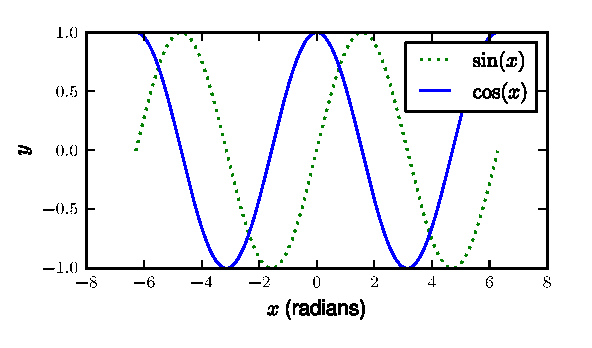
\includegraphics[width=84mm]{fig1.ps}
  %% to include a figure, or
 \vspace{3.5cm}
  %% to leave a blank space
 \caption{An example figure.}
 \label{sample-figure}
\end{figure}
\end{verbatim}

\begin{figure}
%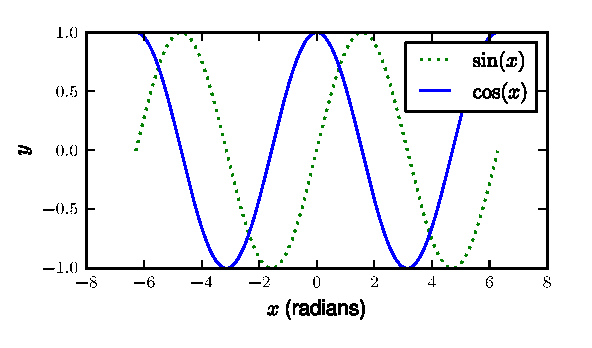
\includegraphics[width=84mm]{fig1.ps}
  %% to include a figure, or
 \vspace{3.5cm}
  %% to leave a blank space
 \caption{An example figure.}
  \label{sample-figure}
\end{figure}

\subsection{Tables}

The {\tt mn2e} class file will cope with most positioning of your
tables and you should not normally use the optional positional
qualifiers on the \verb"table" environment which would override
these decisions. Table captions should be at the top, therefore
the \verb"\caption" command should appear \emph{above} the body of
the table.

The \verb"tabular" environment can be used to produce tables with
single horizontal rules, which are allowed, if desired, at the
head and foot and under the header only. This environment has been
modified for the {\tt mn2e} class in the following ways:
%
\begin{enumerate}
  \item additional vertical space is inserted on either side of a rule;
  \item vertical lines are not produced.
\end{enumerate}
%
Commands to redefine quantities such as \verb"\arraystretch"
should be omitted in general. For example, Table~\ref{symbols} is
produced using the following commands. Note that \verb"\rmn" will
produce a roman character in math mode. There are also \verb"\bld"
and \verb"\itl", which produce bold face and text italic in math
mode.
\begin{table}
 \caption{Radio-band beaming model parameters
          for FSRQs and BL Lacs.}
 \label{symbols}
 \begin{tabular}{@{}lcccccc}
  \hline
  Class & $\gamma _1$ & $\gamma _2$
        & $\langle \gamma \rangle$
        & $G$ & $f$ & $\theta _{\rmn{c}}$ \\
  \hline
  BL Lacs &5 & 36 & 7 & $-4.0$
        & $1.0\times 10^{-2}$ & 10$\degr$ \\
  FSRQs & 5 & 40 & 11 & $-2.3$
        & $0.5\times 10^{-2}$ & 14$\degr$ \\
  \hline
 \end{tabular}

 \medskip
 {\em G} is the slope of the Lorentz factor distribution, i.e.
 $n(\gamma)\propto \gamma ^G$, extending between $\gamma _1$ and
 $\gamma_2$, with mean value $\langle \gamma \rangle$, {\em f\/} is the
 ratio between the intrinsic jet luminosity and the extended, unbeamed
 luminosity, while $\theta_{\rmn{c}}$ is the critical angle separating
 the beamed class from the parent population.
\end{table}
\begin{verbatim}
\begin{table}
 \caption{Radio-band beaming model parameters
          for FSRQs and BL Lacs.}
 \label{symbols}
 \begin{tabular}{@{}lcccccc}
  \hline
  Class & $\gamma _1$ & $\gamma _2$
        & $\langle \gamma \rangle$
        & $G$ & $f$ & $\theta _{\rmn{c}}$ \\
  \hline
  BL Lacs &5 & 36 & 7 & $-4.0$
        & $1.0\times 10^{-2}$ & 10$\degr$ \\
  FSRQs & 5 & 40 & 11 & $-2.3$
        & $0.5\times 10^{-2}$ & 14$\degr$ \\
  \hline
 \end{tabular}

 \medskip
 {\em G} is the slope of the Lorentz factor
   :
 class from the parent population.
\end{table}
\end{verbatim}
%
If you have a table that is to extend over two columns, you need
to use \verb"table*" in a minipage environment, i.e. you can say
%
\begin{verbatim}
\begin{table*}
\begin{minipage}{126mm}
 \caption{Caption which will wrap round to the
          width of the minipage environment.}
 \begin{tabular}{%
      :
 \end{tabular}
\end{minipage}
\end{table*}
\end{verbatim}
%
The width of the minipage should more or less be the width of your
table, so you can only guess on a value on the first pass. The
value will have to be adjusted when your article is typeset in
Times, so do not worry about making it the exact size.

\subsection{Running headlines}

As described above, the title of the article and the author's name (or
authors' names) are used as running headlines at the top of every page.
The headline on left-hand pages can list up to three names; for more than
three use et~al. The \verb"\pagestyle" and \verb"\thispagestyle"
commands should {\em not\/} be used. Similarly, the commands
\verb"\markright" and \verb"\markboth" should not be necessary.


\subsection[]{Typesetting mathematics}\label{TMth}

\subsubsection{Displayed mathematics}

The {\tt mn2e} class file will set displayed mathematics flush with the
left margin, provided that you use the \LaTeXe\ standard of open and closed
square brackets as delimiters. The equation
\[
 \sum_{i=1}^p \lambda_i = \rmn{trace}(\mathbfss{S})
\]
was typeset using the {\tt mn2e} class file with the commands
%
\begin{verbatim}
\[
 \sum_{i=1}^p \lambda_i = \rmn{trace}(\mathbfss{S})
\]
\end{verbatim}
%
Note the difference between the positioning of this equation and of
the following centred equation,
$$ \alpha_{j+1} > \bar{\alpha}+ks_{\alpha} $$
which was wrongly typeset using double dollars as follows:
%
\begin{verbatim}
$$ \alpha_{j+1} > \bar{\alpha}+ks_{\alpha} $$
\end{verbatim}
Please do not use double dollars.

\subsubsection{Bold math italic / bold symbols}

To get bold math italic you should use \verb"\bmath", e.g.
%
\begin{verbatim}
\[
  d(\bmath{s_{t_u}}) = \langle [RM(\bmath{X_y}
  + \bmath{s_t}) - RM(\bmath{x_y})]^2 \rangle
\]
\end{verbatim}
%
to produce:
\[
  d(\bmath{s_{t_u}}) = \langle [RM(\bmath{X_y}
  + \bmath{s_t}) - RM(\bmath{x_y})]^2 \rangle
\]
Working this way, scriptstyle and scriptscriptstyle sizes will take care of
themselves.

\subsubsection{Bold Greek}\label{boldgreek}

Bold lowercase Greek characters can now be obtained by prefixing the normal
(unbold) symbol name with a `b', e.g.\ \verb"\bgamma" gives $\bgamma$. This
rule does not apply to bold \verb"\eta", as this would lead to a name clash
with \verb"\beta". Instead use \verb"\boldeta" for bold eta. Note that
there is no \verb"\omicron" (so there is no \verb"\bomicron"), just use `o'
in math mode for omicron ($o$) and `\verb"\bmath{o}"' for bold omicron
($\bmath{o}$). `\verb"\bmath{}"' can also be used for other Greek
characters.

For bold uppercase Greek, prefix the unbold character name with
%
\verb"\mathbf", e.g.\ \verb"\mathbf\Gamma" gives $\mathbf\Gamma$.
%
Upper and lowercase Greek characters are available in all typesizes.

You can then use these definitions in math mode, as you would normal Greek
characters:
%
\begin{verbatim}
\[
  \balpha_{\bmu} = \mathbf{\Theta} \alpha.
\]
\end{verbatim}
%
%
will produce
%
\[
  \balpha_{\bmu} = \mathbf{\Theta} \alpha.
\]
%

\subsubsection{Upright Greek characters}\label{upgreek}

You can obtain upright Greek characters if you have access to the American
Maths Society Euler fonts (version 2.0), but you may not have these. In
this case, you will have to use the normal math italic symbols and the
typesetter will substitute the corresponding upright characters. You will
make this easier if you can use the macros \verb|\upi|, \verb|\umu| and
\verb|\upartial| etc.\ in your text to indicate the need for upright
characters, together with the {\tt useAMS} global option:
(\verb|\documentclass[useAMS]{mn2e}|). Characters $\upi$, $\umu$ and
$\upartial$ will appear upright only on systems that have the Euler roman
fonts (\verb"eurm"\textit{xx}); characters $\leq$ and $\geq$ appear slanted
only on systems that have the AMS series A fonts (\verb"msam"\textit{xx}).
On systems that do not have these fonts, the standard forms of the
characters appear in the printout; however, they should be correct in the
final typeset paper if the correct \LaTeX\ commands have been used.



\subsubsection{Special symbols}\label{SVsymbols}

The macros for the special symbols in Tables~\ref{mathmode}
and~\ref{anymode} have been taken from the Springer Verlag
`Astronomy and Astrophysics' design, with their permission. They
are directly compatible and use the same macro names. These
symbols will work in all text sizes, but are only guaranteed to
work in text and displaystyles. Some of the symbols will not get
any smaller when they are used in sub- or superscripts, and will
therefore be displayed at the wrong size. Do not worry about this
as the typesetter will be able to sort this out. Authors should
take particular note of the symbols \verb"\la", \verb"\ga",
\verb"\fdg" and \verb"\sun".
%
\begin{table*}
\begin{minipage}{110mm}
\caption{Special symbols which can only be used in math mode.}
\label{mathmode}
\begin{tabular}{@{}llllll}
Input & Explanation & Output & Input & Explanation & Output\\
\hline
\verb"\la"     & less or approx       & $\la$     &
  \verb"\ga"     & greater or approx    & $\ga$\\[2pt]
\verb"\getsto" & gets over to         & $\getsto$ &
  \verb"\cor"    & corresponds to       & $\cor$\\[2pt]
\verb"\lid"    & less or equal        & $\lid$    &
  \verb"\gid"    & greater or equal     & $\gid$\\[2pt]
\verb"\sol"    & similar over less    & $\sol$    &
  \verb"\sog"    & similar over greater & $\sog$\\[2pt]
\verb"\lse"    & less over simeq      & $\lse$    &
  \verb"\gse"    & greater over simeq   & $\gse$\\[2pt]
\verb"\grole"  & greater over less    & $\grole$  &
  \verb"\leogr"  & less over greater    & $\leogr$\\[2pt]
\verb"\loa"    & less over approx     & $\loa$    &
  \verb"\goa"    & greater over approx  & $\goa$\\
\hline
\end{tabular}
\end{minipage}
\end{table*}
%
\begin{table*}
\begin{minipage}{120mm}
\caption{Special symbols which do not have to be used in math
mode.} \label{anymode}
\begin{tabular}{@{}llllll}
Input & Explanation & Output & Input & Explanation & Output\\
\hline
\verb"\sun"      & sun symbol            & $\sun$     &
  \verb"\degr"     & degree                & $\degr$\\[2pt]
\verb"\diameter" & diameter              & \diameter  &
  \verb"\sq"       & square                & \squareforqed\\[2pt]
\verb"\fd"       & fraction of day       & \fd        &
  \verb"\fh"       & fraction of hour      & \fh\\[2pt]
\verb"\fm"       & fraction of minute    & \fm        &
  \verb"\fs"       & fraction of second    & \fs\\[2pt]
\verb"\fdg"      & fraction of degree    & \fdg       &
  \verb"\fp"       & fraction of period    & \fp\\[2pt]
\verb"\farcs"    & fraction of arcsecond & \farcs     &
  \verb"\farcm"    & fraction of arcmin    & \farcm\\[2pt]
\verb"\arcsec"   & arcsecond             & \arcsec    &
  \verb"\arcmin"   & arcminute             & \arcmin\\
\hline
\end{tabular}
\end{minipage}
\end{table*}

\subsection{Bibliography}

References to published literature should be quoted in text by
author and date: e.g. Draine (1978) or (Begelman, Blandford \&
Rees 1984). Where more than one reference is cited having the same
author(s) and date, the letters a,b,c, \ldots\ should follow the
date; e.g.\ Smith (1988a), Smith (1988b), etc. When a three-author
paper is cited, you should list all three authors at the first
citation, and thereafter use `et al.'.


\subsubsection{Use of {\tt natbib}}
If the \verb"usenatbib" global option is specified, Patrick Daly's
\verb"natbib.sty" package will be used for for cross-referencing.
If the \verb"usenatbib" option is specified, citations in the text
should be in one of the following forms (or one of the additional
forms documented within \verb"natbib.sty" itself).

  \begin{itemize}
  \item \verb"\citet{"\textit{key}\verb"}" produces text citations,
  e.g. Jones et al. (1990),
  \item \verb"\citep{"\textit{key}\verb"}" produces citations in parentheses,
  e.g. (Jones et al. 1990),
  \item \verb"\citealt{"\textit{key}\verb"}" produces citations with no parentheses,
  e.g. Jones et al. 1990.
  \end{itemize}
For three-author papers, a full author list can be forced by
putting a \verb"*" just before the \verb"{". To add notes within
the citation, use the form
\verb"\citep["\textit{pre\_reference\_text}\verb"]["\textit{post\_reference\_text}\verb"]{"\textit{key}\verb"}"
(note that either of \textit{pre\_reference\_text} and
\textit{post\_reference\_text} can be blank).

Items in the reference list must be of the form\\
\verb"\bibitem[\protect\citeauthoryear{"\textit{author\_names}\verb"}"\\
 \verb"{"\textit{year}\verb"}]{"\textit{key}\verb"}"
Text of reference ...\\
for one-, two- and multi-author papers, or\\
\verb"\bibitem[\protect\citeauthoryear{"\textit{three\_author\_names}\verb"}"\\
 \verb"{"\textit{first\_author\_etal}\verb"}{"\textit{year}\verb"}]{"\textit{key}\verb"}"
Text of reference ...\\
for three-author papers.

Note that Patrick Daly's package \verb"natbib.sty" is required in
order to use the \verb"usenatbib" option.

We recommend that authors use \verb"natbib.sty" as their standard
cross-referencing package, because of the flexibility in citation
style that it provides.


\subsubsection{The list of references}

The following listing shows some references prepared in the style of
the journal; the code produces the references at the end of this guide.
The following rules apply for the ordering of your references:
%
\begin{enumerate}
  \item if an author has written several papers, some with other authors,
        the rule is that the single-author papers precede the two-author
        papers, which, in turn, precede the multi-author papers;
  \item within the two-author paper citations, the order is determined
        by the second author's surname, regardless of date;
  \item within the multi-author paper citations, the order is
        chronological, regardless of authors' surnames.
\end{enumerate}
%
\begin{verbatim}
\begin{thebibliography}{}
  \bibitem[\protect\citeauthoryear{Butcher}{1992}]{bu}
    Butcher J., 1992, Copy-editing: The Cambridge
    Handbook, 3rd edn. Cambridge Univ. Press,
    Cambridge
  \bibitem[\protect\citeauthoryear{The Chicago Manual}%
    {1982}]{ch} The Chicago Manual of Style, 1982.
    Univ. Chicago Press, Chicago
  \bibitem[\protect\citeauthoryear{Blanco}{1991}]{bl}
    Blanco P., 1991, PhD thesis, Edinburgh
    University
  \bibitem[\protect\citeauthoryear{Brown \& Jones}%
    {1989}]{bj} Brown A. B., Jones C. D., 1989,
    in Robinson E. F., Smith G. H., eds,
    Proc. IAU Symp. 345, Black Dwarfs.
    Kluwer, Dordrecht, p. 210
  \bibitem[\protect\citeauthoryear{Edelson}{1987}]{ed}
    Edelson R. A., 1987, ApJ, 313, 651
  \bibitem[\protect\citeauthoryear{Knuth}{1998}]{kn}
    Knuth D. E., 1998, The \TeX book. Addison-Wesley,
    Reading, MA
  \bibitem[\protect\citeauthoryear{Kopka \& Daly}%
    {1999}]{kd} Kopka H., Daly P. W., 1999, A Guide
    to \LaTeX, 3rd edn. Addison-Wesley, Harlow
  \bibitem[\protect\citeauthoryear{Lamport}{1986}]{la}
    Lamport L., 1986, \LaTeX: A Document
    Preparation System. Addison--Wesley, New York
  \bibitem[\protect\citeauthoryear{Mirabel \& Sanders}%
    {1989}]{ms} Mirabel I. F., Sanders D. B., 1989,
    ApJ, 340, L53
  \bibitem[\protect\citeauthoryear{Misner et al.}%
    {1973}]{mtw} Misner C. W., Thorne K. S.,
    Wheeler J. A., 1973, Gravitation.
    Freeman, San Francisco
  \bibitem[\protect\citeauthoryear{Sopp \& Alexander}%
    {1991}]{sa} Sopp H. M., Alexander P., 1991,
    MNRAS, 251, 112
  \bibitem[\protect\citeauthoryear{Stella \& Campana}%
    {1991}]{sc} Stella L., Campana S., 1991, in
    Treves A., Perola G. C., Stella L., eds,
    Iron Line Diagnostic in X-ray Sources.
    Springer--Verlag, Berlin, p. 230
\end{thebibliography}
\end{verbatim}
%
Each entry takes the form
%
\begin{verbatim}
\bibitem[\protect\citeauthoryear{Author(s)}%
  {Date}]{tag} Bibliography entry
\end{verbatim}
%
where \verb"Author(s)" should be the author names as they are
cited in the text, \verb"Date" is the date to be cited in the
text, and \verb"tag" is the tag that is to be used as an argument
for the vatious \verb"\cite" commands. \verb"Bibliography entry"
should be the material that is to appear in the bibliography,
suitably formatted.

Please, wherever possible, supply the formatted .bbl file of your
reference list rather than the `raw' .bib file(s).

\subsection{Appendices}

The appendices in this guide were generated by typing:
%
\begin{verbatim}
\appendix
\section{For authors}
     :
\section{For editors}
\end{verbatim}
%
You only need to type \verb"\appendix" once. Thereafter, every
\verb"\section" command will generate a new appendix which will be
numbered A, B, etc. Figures and tables that appear in the
Appendices should be called Fig. A1, Table A1, etc.


\section[]{Example of section heading with\\*
  S{\sevensize\bf MALL} C{\sevensize\bf APS},
  \lowercase{lowercase}, \textbfit{italic},
  and bold\\* Greek such as
  $\bmu^{\bkappa}$}\label{headings}

%
There are at least two ways of achieving this section head. The first
involves the use of \verb"\boldmath". You could say:
%
\begin{verbatim}
\section[]{Example of section heading with\\*
  S{\sevensize\bf MALL} C{\sevensize\bf APS},
  \lowercase{lowercase}, \textbfit{italic},
  and bold\\* Greek such as
  \mbox{\boldmath{$\mu^{\kappa}$}}}
\end{verbatim}
%
Many implementations of \LaTeX\ do not support \verb"\boldmath" at 9pt,
so you may need to use the bold Greek characters as described in
Section~\ref{boldgreek}, and typeset the section head as follows:
%
\begin{verbatim}
\section[]{Example of section heading with\\*
  S{\sevensize\bf MALL} C{\sevensize\bf APS},
  \lowercase{lowercase}, \textbfit{italic},
  and bold\\* Greek such as
  $\bmu^{\bkappa}$}
\end{verbatim}
%
%
Was produced with:
%
\begin{verbatim}
\section[]{Example of section heading with\\*
  S{\sevensize MALL} C{\sevensize APS},
  \lowercase{lowercase}, \textbfit{italic},
  and bold\\* Greek such as
  $\bmu^{\bkappa}$}
\end{verbatim}
%

\begin{thebibliography}{}
  \bibitem[\protect\citeauthoryear{Butcher}{1992}]{bu}
    Butcher J., 1992, Copy-editing: The Cambridge
    Handbook, 3rd edn. Cambridge Univ. Press,
    Cambridge
  \bibitem[\protect\citeauthoryear{The Chicago Manual}%
    {1982}]{ch} The Chicago Manual of Style, 1982.
    Univ. Chicago Press, Chicago
  \bibitem[\protect\citeauthoryear{Blanco}{1991}]{bl}
    Blanco P., 1991, PhD thesis, Edinburgh
    University
  \bibitem[\protect\citeauthoryear{Brown \& Jones}%
    {1989}]{bj} Brown A. B., Jones C. D., 1989,
    in Robinson E. F., Smith G. H., eds,
    Proc. IAU Symp. 345, Black Dwarfs.
    Kluwer, Dordrecht, p. 210
  \bibitem[\protect\citeauthoryear{Edelson}{1987}]{ed}
    Edelson R. A., 1987, ApJ, 313, 651
  \bibitem[\protect\citeauthoryear{Knuth}{1998}]{kn}
    Knuth D. E., 1998, The \TeX book. Addison-Wesley, Reading, MA
  \bibitem[\protect\citeauthoryear{Kopka \& Daly}{1999}]{kd}
    Kopka H., Daly P. W., 1999, A Guide to \LaTeX, 3rd edn. Addison-Wesley,
    Harlow
  \bibitem[\protect\citeauthoryear{Lamport}{1986}]{la}
    Lamport L., 1986, \LaTeX: A Document
    Preparation System. Addison--Wesley, New York
  \bibitem[\protect\citeauthoryear{Mirabel \& Sanders}%
    {1989}]{ms} Mirabel I. F., Sanders D. B., 1989,
    ApJ, 340, L53
  \bibitem[\protect\citeauthoryear{Misner et al.}%
    {1973}]{mtw} Misner C. W., Thorne K. S.,
    Wheeler J. A., 1973, Gravitation.
    Freeman, San Francisco
  \bibitem[\protect\citeauthoryear{Sopp \& Alexander}%
    {1991}]{sa} Sopp H. M., Alexander P., 1991,
    MNRAS, 251, 112
  \bibitem[\protect\citeauthoryear{Stella \& Campana}%
    {1991}]{sc} Stella L., Campana S., 1991, in
    Treves A., Perola G. C., Stella L., eds,
    Iron Line Diagnostic in X-ray Sources.
    Springer--Verlag, Berlin, p. 230
\end{thebibliography}


\appendix
\section{For authors}

Table~\ref{authors} is a list of design macros which are unique to
the Monthly Notices class and style files. The list displays each
macro's name and description.

For detailed guidelines on style, authors are referred to the
journal web page. Adherence to correct style from the start will
obviously save time and effort later on, in terms of fewer proof
corrections.  The notes given on the journal web page relate to
common style errors found in  Monthly Notices manuscripts, and are
{\it not\/} intended to be exhaustive. Please see the editorials
in issues 257/2 and 260/1, as well as any recent issue of the
journal, for more details.


\begin{table*}
\begin{minipage}{155mm}
\caption{Authors' notes.}
\label{authors}
\begin{tabular}{@{}ll}
\verb"\title[optional short title]{long title}"
                    & short title used in running head\\
\verb"\author[optional short author(s)]{long author(s)}"
                    & short author(s) used in running head\\
\verb"\newauthor"   & starts a new line in the author environment\\
\verb"\begin{abstract}...\end{abstract}"& for abstract on titlepage\\
\verb"\begin{keywords}...\end{keywords}"& for keywords on titlepage\\
\verb"\nokeywords"  & if there are no keywords on titlepage\\
\verb"\begin{figure*}...\end{figure*}" & for a double spanning figure in two-column mode\\
\verb"\begin{table*}...\end{table*}" & for a double spanning table in
                                       two-column mode\\
\verb"\plate{Opposite p.~812, MNRAS, {\bf 261}}"
                  & used with \verb"\thispagestyle{plate}" for plate pages\\
\verb"\contcaption{}" & for continuation figure and table captions\\
\verb"\bmath{math text}" & Bold math italic / symbols.\\
\verb"\textbfit{text}", \verb"\mathbfit{text}" & Bold text italic
   (defined in the preamble of \verb"mnsample.tex").\\
\verb"\textbfss{text}", \verb"\mathbfss{text}" & Bold text sans serif
   (defined in the preamble of \verb"mnsample.tex").\\
\end{tabular}
\end{minipage}
\end{table*}


\section{For editors}

The additional features shown in Table~\ref{editors} may be used
for production purposes. The most commonly used of these is \verb"\bsp",
which produces the `This paper $\ldots$' statement. This should be
placed at the end of the document.

\begin{table*}
\begin{minipage}{155mm}
\caption{Editors' notes.}
\label{editors}
\begin{tabular}{@{}lp{270pt}}
\verb"\pagerange{000--000}"& for catchline, note use of en-rule\\
\verb"\pagerange{L00--L00}"& for letters option, used in catchline\\
\verb"\volume{000}" & volume number, for catchline\\
\verb"\pubyear{0000}" & publication year, for catchline\\
\verb"\journal" & replace the whole catchline at one go\\
\verb"[doublespacing]" & documentstyle option for doublespacing\\
\verb"[galley]" & documentstyle option for running to galley\\
\verb"[landscape]" & documentstyle option for landscape illustrations\\
\verb"[letters]" & documentstyle option, for short communications
                   (adds L to folios)\\
\verb"[onecolumn]" & documentstyle option for one-column \\
\verb"[referee]" & documentstyle option for 12/20pt, single col,
                   39pc measure\\
\verb"\bsp" & typesets the final phrase `This paper has been typeset
              from a\\
            & \TeX/\LaTeX\ file prepared by the author.'\\
\end{tabular}
\end{minipage}
\end{table*}


%%%%%%%%%%%%%%%%%%%%%%%%%%%%%%%%%%%%

\makeatletter
% define \thebiblio (same as thebibliography, but
% without the section heading)
\def\thebiblio#1{%
 \list{}{\usecounter{dummy}%
         \labelwidth\z@
         \leftmargin 1.5em
         \itemsep \z@
         \itemindent-\leftmargin}
 \reset@font\small
 \parindent\z@
 \parskip\z@ plus .1pt\relax
 \def\newblock{\hskip .11em plus .33em minus .07em}
 \sloppy\clubpenalty4000\widowpenalty4000
 \sfcode`\.=1000\relax
}
\let\endthebiblio=\endlist
\makeatother


\section{Troubleshooting}

Authors may from time to time encounter problems with the  preparation
of their papers in \TeX/\LaTeX. The appropriate  action  to
take will depend on the nature of the problem -- the following is
intended to act as a guide.
%
\begin{enumerate}
\item If a problem is with \TeX/\LaTeX\ itself, rather than with the
actual macros, please refer to the appropriate handbooks for
initial advice \citep{kd,kn}. If the solution cannot be found
after discussion with colleagues, and you suspect that the problem
lies with the macros, then please contact the RAS Journal
Production team at Blackwell Publishing, 23 Ainslie Place,
Edinburgh EH3 6AJ, UK [Tel: +44 (0)131 226 7232; Fax: +44 (0)131
226 3803]. The Blackwell Publishing office may also be reached
using the journal e-mail address (mnr@blacksci.co.uk). Please
provide precise details of the problem (what you were trying to do
-- ideally, include examples of source code as well -- and what
exactly happened; what error message was received).

\item Problems with page make-up, particularly in the two-column
mode (e.g.\ large spaces between paragraphs, or under headings or figures;
uneven columns; figures/tables appearing out of order). Please do {\it
not\/} attempt to remedy these yourself using `hard' page make-up commands
-- the typesetters will sort out such problems during the typesetting
process. (You may, if you wish, draw attention to particular problems when
submitting the final version of your paper.)

\item If a required font is not available at your site, allow \TeX\
to substitute the font and report the problem on your FTP submission form.

\item If you choose to use \verb"\boldmath", you may find that boldmath has
not been defined locally for use with a particular size of font. If this is
the case, you will get a message that reads something like:
%
\begin{verbatim}
LaTeX Warning: No \boldmath typeface in this size,
using \unboldmath on input line 44.
\end{verbatim}

If you get this message, you are advised to use the alternative described
in this guide for attaining bold face math italic characters,
i.e.\ \verb"\bmath{...}".
\end{enumerate}


\label{here}

\subsection{Fixes for coding problems}

The new versions of the class file and macros have been designed
to minimize the need for user-defined macros to  create  special
symbols. Authors are urged, wherever possible, to use the
following coding rather than create their own. This will minimize
the danger of author-defined macros being accidentally
`overridden' when the paper is typeset in 9/11~pt Times Roman (see
Section~\ref{TMth}, `Typesetting  mathematics', in the \LaTeX\
author guide).
%
\begin{enumerate}
\item Fonts in sections and paper titles. The following are  examples
of styles that sometimes prove difficult to code.
\end{enumerate}


\subsubsection*{P\lowercase{aper titles}}

\boxit{\huge\bf
  A survey of \textit{IRAS} galaxies at
  $\bmath{\delta > 50\degr}$}
%
is produced by:
%
\begin{verbatim}
\title[A survey of {\rm IRAS} galaxies at
       $\delta > 50\degr$]
  {A survey of \textit{IRAS} galaxies at
   $\bmath{\delta > 50\degr}$}
\end{verbatim}
\bigskip

\boxit{\huge\bf Observations of compact H\,{\Large\bf II} regions}
%
is produced by:
%
\begin{verbatim}
\title[Observations of compact H\,{\normalsize
       \it II} regions]
  {Observations of compact H\,{\Large\bf II}
   regions}
\end{verbatim}


\subsubsection*{S\lowercase{ection headings}}

\boxit{\bf 1\quad THE \textit{IRAS} DATA FOR
  $\bmath{\delta > 50\degr}$}
%
is produced by:
%
\begin{verbatim}
\section[]{The \textit{IRAS} data for
  $\bmath{\delta > 50\degr}$
\end{verbatim}
\bigskip

\boxit{\bf 2\quad H\,{\sevensize\bf II} GALAXIES AT
  $\bmath{\lowercase{z} > 1.6}$}
%
is produced by:
%
\begin{verbatim}
\section[]{H\,{\sevensize\bf II} galaxies at
  $\bmath{\lowercase{z} > 1.6}$}
\end{verbatim}


\subsubsection*{S\lowercase{ubsection headings}}

\boxit{\bf 2.1\quad The \textit{IRAS} data for
  $\bmath{\delta > 50\degr}$: galaxies
  at $\bmath{z > 1.5}$}
%
is produced by:
%
\begin{verbatim}
\subsection[]{The \textit{IRAS} data for
  $\bmath{\delta > 50\degr}$: galaxies
  at $\bmath{z > 1.5}$}
\end{verbatim}
\bigskip

\boxit{\bf 2.2\quad Observations of compact H\,{\sevensize\bf II} regions}
%
is produced by:
%
\begin{verbatim}
\subsection[]{Observations of compact
  H\,{\sevensize\bf II} regions}
\end{verbatim}
\bigskip

\boxit{\it 2.2.1\quad A survey of radio galaxies for
  $\delta > 50\degr$}
%
is produced by:
%
\begin{verbatim}
\subsubsection[]{A survey of radio galaxies for
  $\delta > 50\degr$}
\end{verbatim}
\bigskip

\boxit{\it 2.2.2\quad Determination of $T_{\rm eff}$ in compact
  H\,{\sevensize\it II} regions}
%
is produced by:
%
\begin{verbatim}
\subsubsection[]{Determination of $T_{\rm eff}$ in
  compact H\,{\sevensize\it II} regions}
\end{verbatim}
\bigskip

\begin{enumerate}
\stepcounter{enumi}

\item Small capitals and other unusual fonts in table and figure captions:
\par\smallskip
\boxit{\small {\bf Figure 1.} Profiles of the H$\alpha$ and
  N\,{\sc iii} lines observed.}
%
is produced by:
%
\begin{verbatim}
\caption{Profiles of the H$\alpha$ and
  N\,{\sc iii} lines observed.}
\end{verbatim}

\item Multiple author lists (to get the correct vertical spacing
and wraparound on the title page of a multiple-author paper).
\par\smallskip

\boxit{\huge\bf
  The variation in the\newline
  strength of low-$\bmath{l}$ solar
  p modes: 1981--2
\medskip

\LARGE
  Y. Elsworth, R. Howe, G.R. Isaac, C.~P. McLeod,
  B.~A. Miller, R. New,
  C.~C. Speake and S.~J. Wheeler}
%
is produced by:
%
\begin{verbatim}
\title[The variation in the strength of low-$l$
  solar p modes: 1981--2]%
  {The variation in the strength of
  low-$\bmath{l}$ solar
  p modes: 1981--2}

\author[Y. Elsworth et al.]
  {Y. Elsworth, R. Howe, G.R. Isaac, \newauthor
  C.~P. McLeod, B.~A. Miller, R. New, \newauthor
  C.~C. Speake and S.~J. Wheeler}
\end{verbatim}

\item Ionized species (as used in the examples above). The correct
style calls for the use of small capitals and a thin space after
the symbol for the element: e.g.\ for \hbox{H\,{\sc ii}}, use the
code \verb"\mbox{H\,{\sc ii}}". The use of the \verb"\mbox" will
stop the H and the {\sc ii} being separated.

\item Lower case greek pi ($\pi$), mu ($\mu$) and partial ($\partial$).
In certain circumstances, the \textit{Monthly Notices} style calls
for these to be roman [when pi is used to denote the constant
3.1415$\ldots$, mu is used to denote `micro' in a unit (e.g.\
$\umu$m, $\umu$Jy), and partial is a differential symbol]. See
Section~\ref{upgreek} for instructions.

\item Decimal degrees, arcmin, arcsec, hours, minutes and seconds.
The symbol needs to be placed vertically above the decimal point.
For example, the sentence
%
\begin{quote}
The observations were made along position angle 120\fdg 5,
starting from the central coordinates
$\rmn{RA}(1950)=19^{\rmn{h}}~22^{\rmn{m}}~18\fs2$,
$\rmn{Dec.}~(1950)=45\degr~18\arcmin~36\farcs 4$
\end{quote}
%
uses the following coding:
%
\begin{verbatim}
The observations were made along position angle
120\fdg 5, starting from the central coordinates
$\rmn{RA}(1950)=19^{\rmn{h}} 22^{\rmn{m}} 18\fs2$,
$\rmn{Dec.}~(1950)=45\degr 18\arcmin 36\farcs 4$
\end{verbatim}

\item The correct coding for the prime symbol~\arcmin\ is
\verb"\arcmin", and that for \arcsec\ is \verb"\arcsec"; see the
two tables on special symbols. Note that these symbols should
\emph{only} be used for coordinates. The words `arcmin' and
`arcsec' should be used for units (e.g. `4.5-arscec resolution').

\item N-rules, hyphens and minus signs (see the instructions for
authors on the journal web page for
correct usage). To create the correct symbols in the sentence
%
\begin{quote}
The high-resolution observations were made along a line at an
angle of $-15\degr$ (east from north) from the axis of the jet,
which runs north--south
\end{quote}
you would use the following code:
%
\begin{verbatim}
The high-resolution observations were made along
a line at an angle of $-15\degr$ (east from north)
from the axis of the jet, which runs north--south
\end{verbatim}

\item Vectors and matrices should be bold italic and bold sans
serif respectively. To create the correct fonts for the vector $\bmath{x}$
and the matrix \textbfss{P}, you should use \verb"$\bmath{x}$" and
\verb"\textbfss{P}" respectively; \verb"\mathbfss" is for use in
math mode. Bold face text italic can be obtained by using
\verb"\textbfit{..}" and \verb"\mathbfit{..}" for math mode.

\item Bold italic superscripts and subscripts. To get  these
to  come  out  in the correct font and the right  size,
you need to use \verb"\bmath". You can create the output
$\bmath{k_x}$ by typing \verb"$\bmath{k_x}$".
Try to avoid using \LaTeX\ commands to determine script sizes
that are already  defined in the style file. For example, macros such as
%
\begin{verbatim}
\newcommand{\th}{^\mbox{\tiny th}}
\end{verbatim}
%
are generating extra work;
%
\begin{verbatim}
\newcommand{\th}{^{th}}
\end{verbatim}
%
will do, and  will get  the  size  of the superscript right whether
in  main  text, tables or captions (the use of \verb"\tiny" over-rides
the style  file).
Also, the \verb"\mbox" is not necessary, as \TeX\ will not split a
superscript/subscript from its variable at a line break.

\item Calligraphic letters (uppercase only).
%
Normal uppercase calligraphic can be produced with \verb"\mathcal" as
normal (in math mode). Bold calligraphic can be produced with
\verb"\bmath". e.g.\ \verb"$\bmath{\mathcal A}$" gives $\bmath{\mathcal
A}$.
%

\item Automatic scaling of brackets. The codes \verb"\left" and
\verb"\right" should  be used to scale brackets automatically to
fit the equation being set. For example, to get
\[
  v = x \left( \frac{N+2}{N} \right)
\]
use the code
%
\begin{verbatim}
\[
  v = x \left( \frac{N+2}{N} \right)
\]
\end{verbatim}

\item Roman font in equations. It is often necessary to make some
symbols roman in an equation (e.g.\ units, subscripts). For  example,
to get the following output:
\[
  \sigma \simeq (r/13~h^{-1}~\rmn{Mpc})^{-0.9},
  \qquad \omega = \frac{N-N_{\rmn{s}}}{N_{\rmn{R}}},
\]
you should use:
%
\begin{verbatim}
\[
  \sigma \simeq (r/13~h^{-1}~\rmn{Mpc})^{-0.9},
  \qquad \omega=\frac{N-N_{\rmn{s}}}{N_{\rmn{R}}},
\]
\end{verbatim}

\item Continuation figure and table captions.
See Section~\ref{contfigtab}.
\end{enumerate}


\subsection{Springer-Verlag macro names}

These have been incorporated from the Astronomy \& Astrophysics \LaTeX\
style file, to aid in the creation of various commonly used
astronomical symbols. Please see Section~\ref{SVsymbols} for details.

%%%%%%%%%%%%%%%%%%%%%%%%%%%%%%%%%%%%

% \bsp % ``This paper has been produced using the ...''

\label{lastpage}

\end{document}
